\documentclass{article}
\usepackage[utf8]{inputenc}
\usepackage{enumerate}
\usepackage{amsmath}
\usepackage{amssymb}
\usepackage{amsfonts}
\usepackage{amstext}
\usepackage{amsthm}
\usepackage{mathtools}
\usepackage{tikz}
\usepackage{amsmath}
\usepackage{cancel}
\DeclarePairedDelimiter{\ceil}{\lceil}{\rceil}
\title{Calculus III Midterm 1 Practice}
\author{Eddie Ozuna,Tyler Franklin}

\begin{document}
\maketitle
\section{.}
\begin{enumerate}[a.]
	\item \textbf{What is the geometric significance of the dot product? }\\
	\\
Two vectors are orthogonal(Perpendicular) if and only if the result of the dot product is equal to zero.\\\\
$\vec{u} = <u_{1},u_{2},u_{3}>\hspace{.4cm}\vec{v} = <v_{1},v_{2},v_{3}>$\\
\\
Reminder in how to perform the dot product:\\
\\
$\vec{u} \cdot \vec{v} = (u_{1} \cdot v_{1}) + (u_{2} \cdot v_{2}) + (u_{3} \cdot v_{3}) $\\
\\
Another Approach in how to perform the dot product:\\
\\
$\vec{u} \cdot \vec{v} =  \mid\vec{u}\mid\mid\vec{v}\mid\cos(\theta)$\\
\\
$\mid\vec{u}\mid = \sqrt{u_{1}\hspace{.001cm}^{2}+u_{2}\hspace{.001cm}^{2}+u_{3}\hspace{.001cm}^{2}}$\\
\\
$\mid\vec{v}\mid = \sqrt{v_{1}\hspace{.001cm}^{2}+v_{2}\hspace{.001cm}^{2}+v_{3}\hspace{.001cm}^{2}}$\\
\\
$\theta$ = The angle between the two vectors $\vec{u}$ and $\vec{v}$
\end{enumerate}
\begin{enumerate}[b.]
	\item \textbf{Why does the dot product have such geometric significance? Can you prove it? Hint: Remember the Pythagorean Theorem and its degeneration into the Law of Cosines. Can
you draw a picture to describe the scenario? }\\
	\\
	The dot product take into consideration the angle between them and them take the cosine of that angle. Any vectors that are orthogonal has a angle of 90 degree between them so if you take the cosine of 90 the result is zero and anything multiply with zero of course is zero.\\
	
	Derivation: Law of Cosine\\
	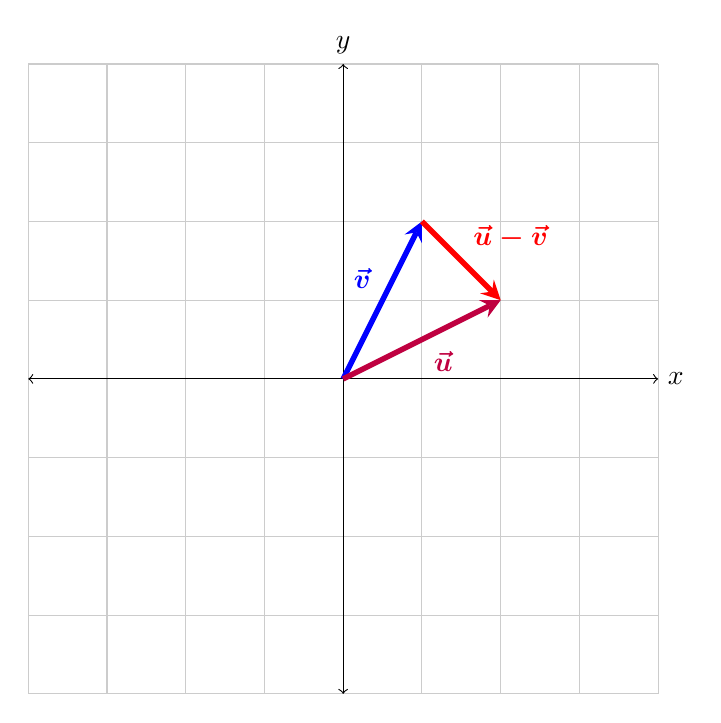
\begin{tikzpicture}
  \draw[thin,gray!40] (-4,-4) grid (4,4);
  \draw[<->] (-4,0)--(4,0) node[right]{$x$};
  \draw[<->] (0,-4)--(0,4) node[above]{$y$};
  \draw[line width=2pt,blue,-stealth](0,0)--(1,2) coordinate (VecV) node[midway,auto]{$\boldsymbol{\vec{v}}$};
  \draw[line width=2pt,purple,-stealth](0,0)--(2,1) coordinate (VecU) node[midway,auto,swap]{$\boldsymbol{\vec{u}}$};
  \draw[line width=2pt,red,-stealth](1,2)--(2,1) node[midway,auto]{$\boldsymbol{\vec{u}-\vec{v}}$};
  
\end{tikzpicture}\\
\\
	$\mid\vec{u}-\vec{v}\mid^{2} = \mid\vec{u}\mid^{2} + \mid\vec{v}\mid^{2}-\hspace{.1cm}2\mid\vec{u}\mid\cdot\mid\vec{v}\mid\cos(\theta)$\\
\\
$\cancel{\mid\vec{u}\mid^{2}}-\hspace{.1cm}2\vec{v}\cdot\vec{u}\hspace{.1cm}+\cancel{\mid\vec{v}\mid^{2}}=\cancel{\mid\vec{u}\mid^{2}} + \cancel{\mid\vec{v}\mid^{2}}-2\mid\vec{u}\mid\cdot\mid\vec{v}\mid\cos(\theta)$\\
\\
$\cancel{-2}\vec{v}\cdot\vec{u} = \cancel{-2}\mid\vec{u}\mid\cdot\mid\vec{v}\mid\cos(\theta)$\\
\\
$\vec{v}\cdot\vec{u} = \mid\vec{u}\mid\cdot\mid\vec{v}\mid\cos(\theta)$\\
\end{enumerate}
\end{document}

